\begin{appendices}
%\appendix
\renewcommand\thefigure{\thesection.\arabic{figure}} 
\setcounter{figure}{0}

%\section*{Appendices}
%\addcontentsline{toc}{chapter}{Appendices}
\renewcommand{\thesection}{\Alph{section}}

\definecolor{codegreen}{rgb}{0,0.6,0}
\definecolor{codegray}{rgb}{0.5,0.5,0.5}
\definecolor{codepurple}{rgb}{0.58,0,0.82}
\definecolor{backcolour}{rgb}{0.95,0.95,0.92}
\definecolor{deepred}{rgb}{0.6,0,0}
 
\lstdefinestyle{mystyle}{
    backgroundcolor=\color{backcolour},   
    commentstyle=\color{codegreen},
    keywordstyle=\color{blue},
    numberstyle=\tiny\color{codegray},
    stringstyle=\color{codepurple},
    basicstyle=\footnotesize,
    breakatwhitespace=false,         
    breaklines=true,                 
    captionpos=b,                    
    keepspaces=true,                 
    numbers=left,                    
    numbersep=5pt,                  
    showspaces=false,                
    showstringspaces=false,
    showtabs=false,                  
    tabsize=2
}
 
\lstset{style=mystyle}

% Can input the GANTT chart as either pdf or image (commented below)
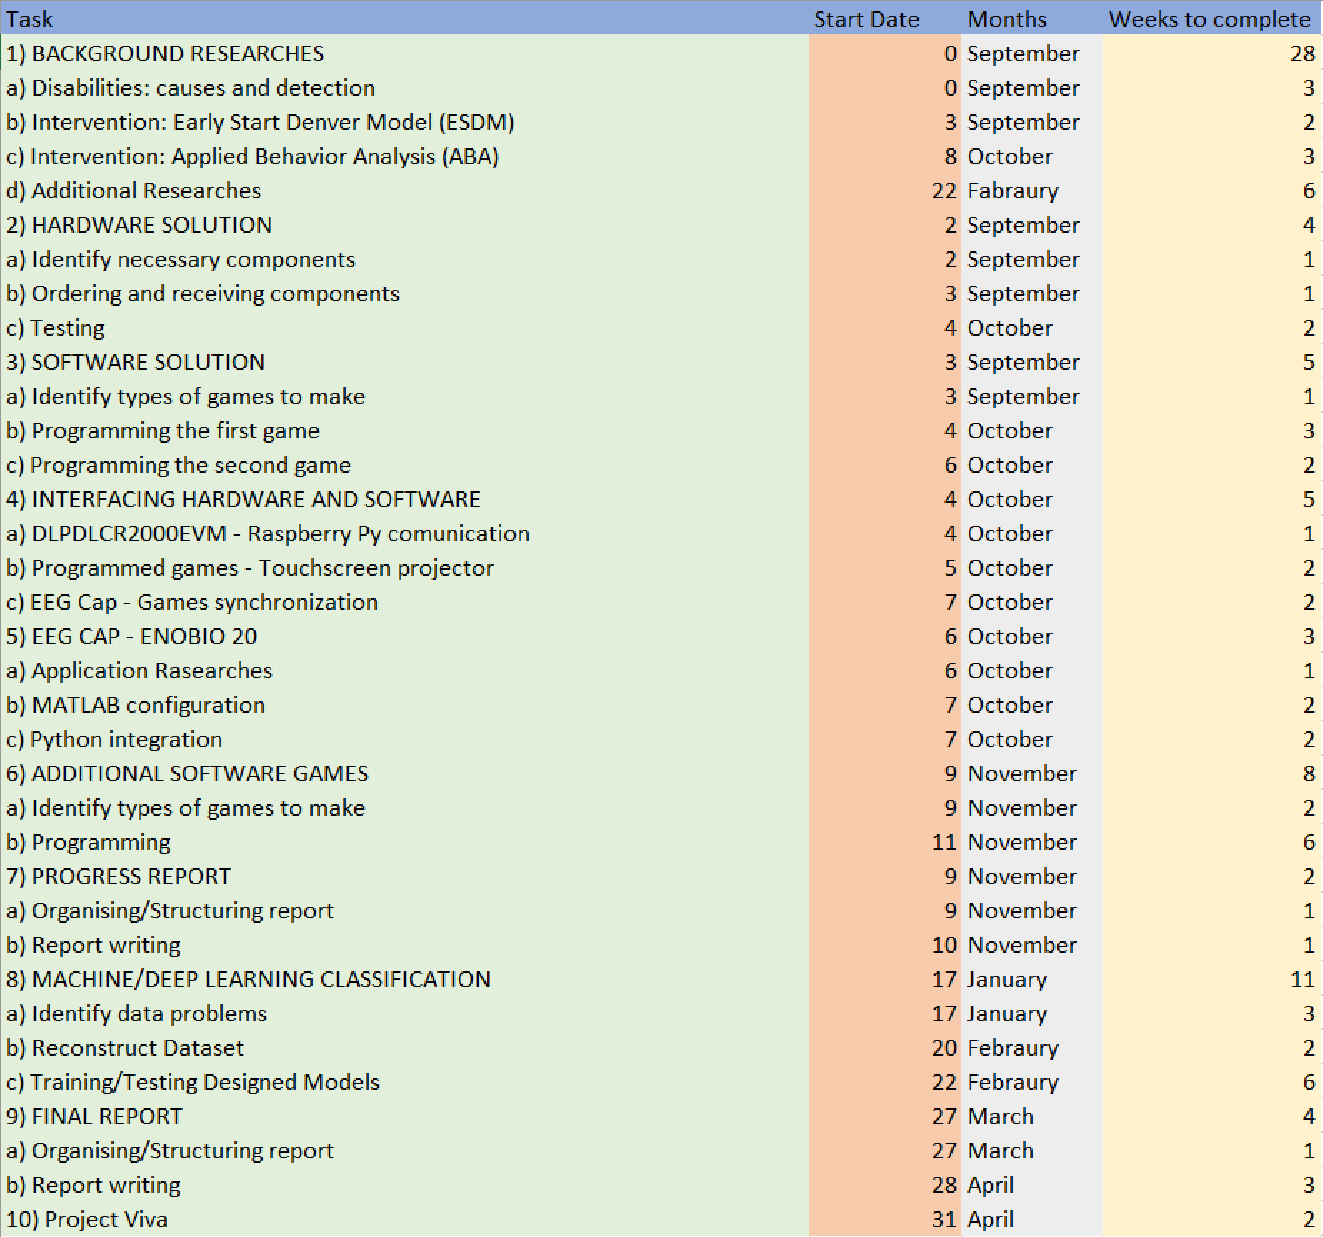
\includepdf[pages=-,pagecommand={\section{Project Management}\null\vfill\captionof{figure}{First and Second Semester Gantt Chart Data}},noautoscale=true,offset=0 -10, scale=0.7]{images/g1.pdf}
%\section{Gantt Chart}
% \begin{figure}[ht!]%
%     \centering
%     %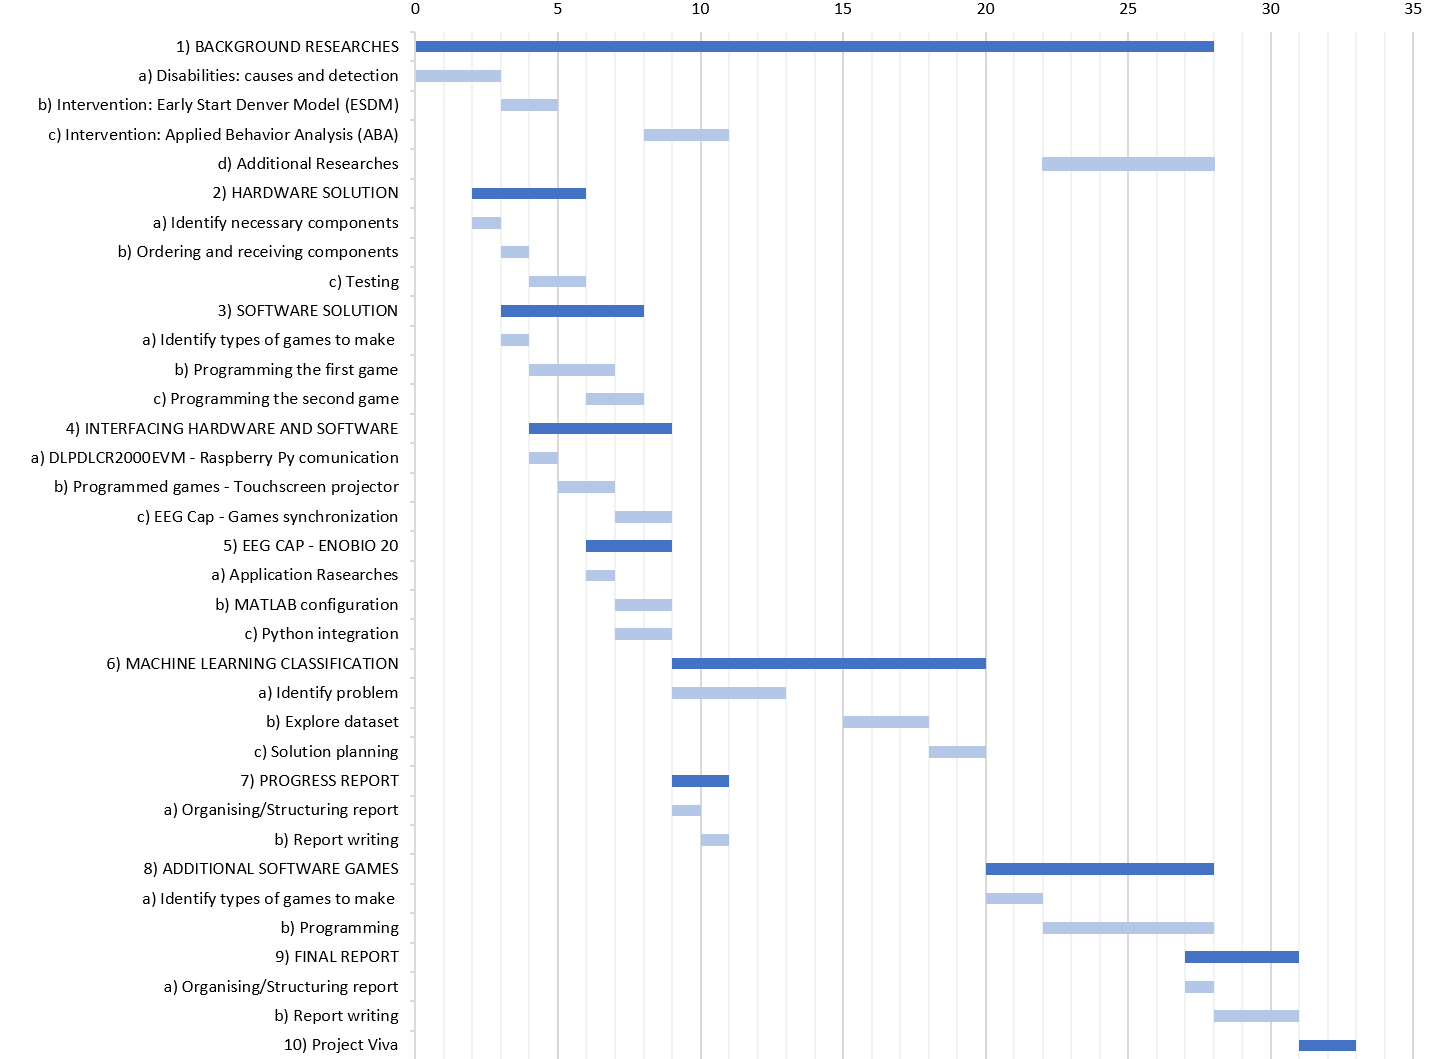
\includegraphics[width=18cm]{images/GANTT}%
%     \caption{First and Second Semester Gantt Chart}%
% \end{figure}
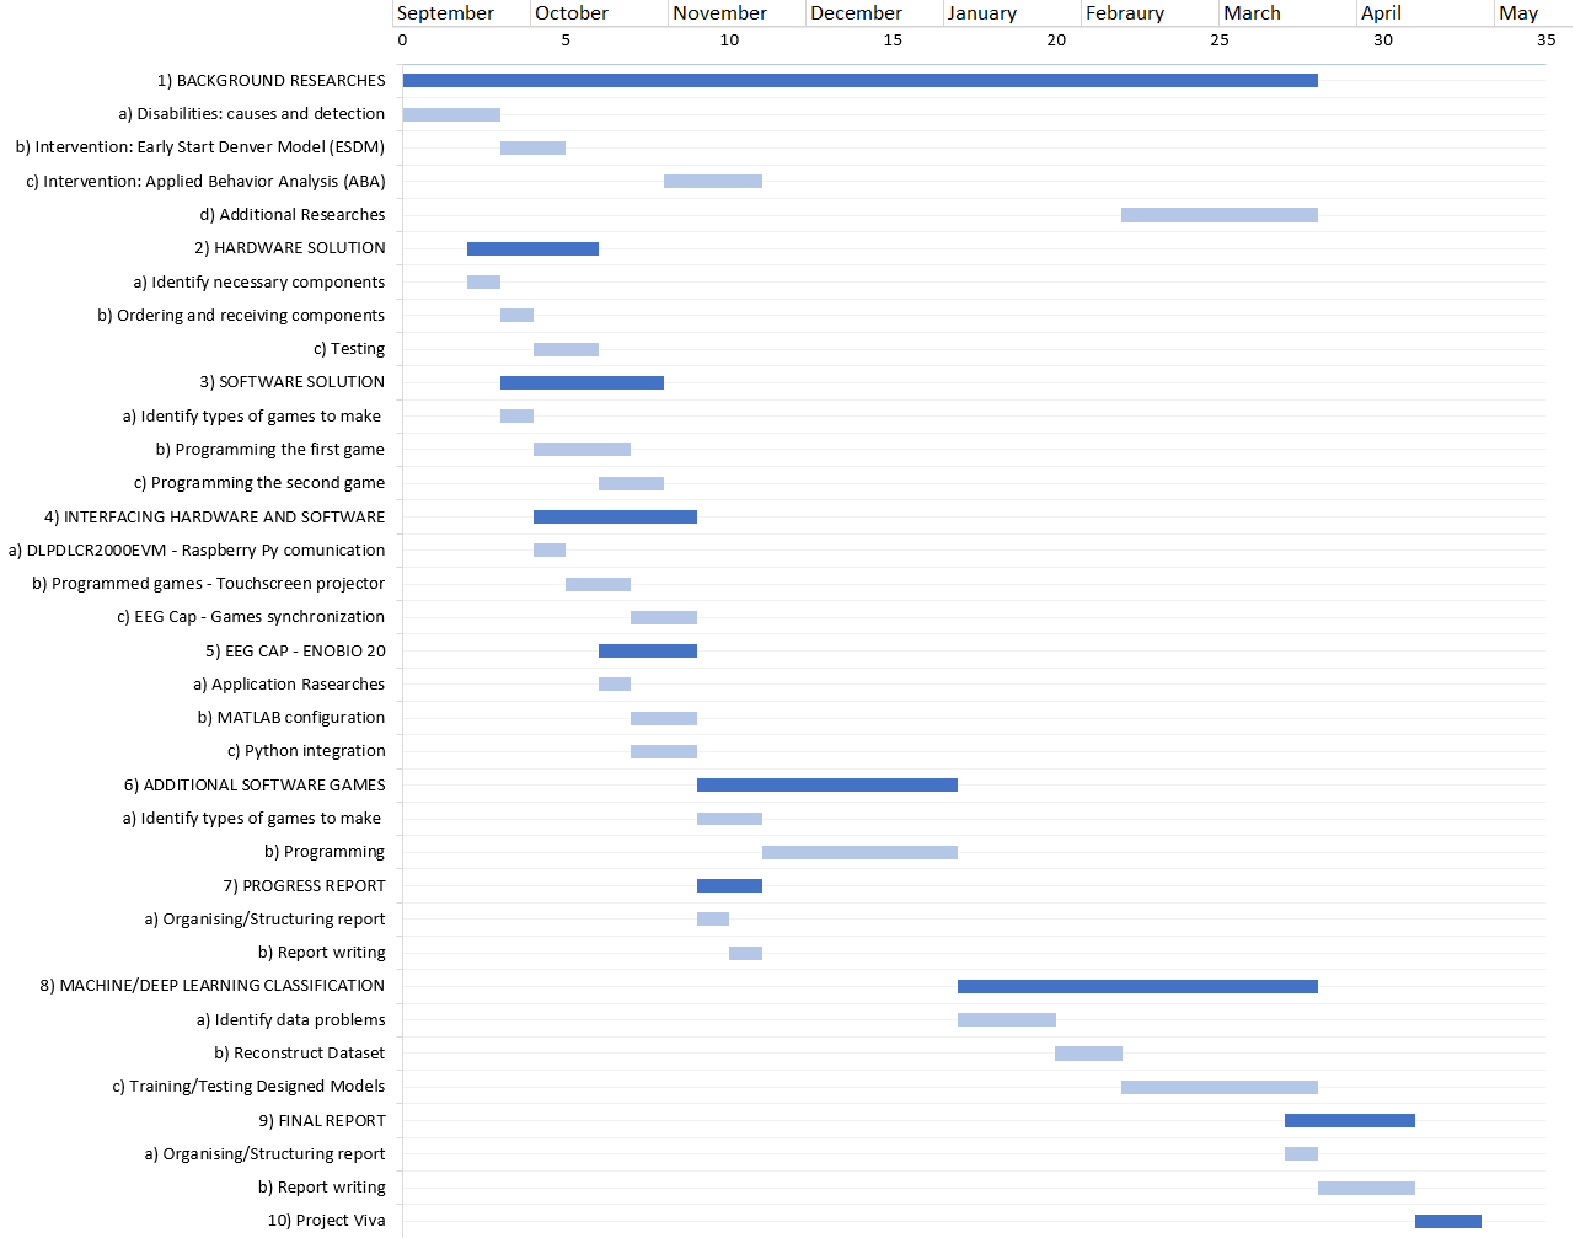
\includepdf[pages=-,pagecommand={\null\vfill\captionof{figure}{Planned Gantt Chart}},noautoscale=true,offset=0 -10, scale=0.65]{images/g2p.pdf}

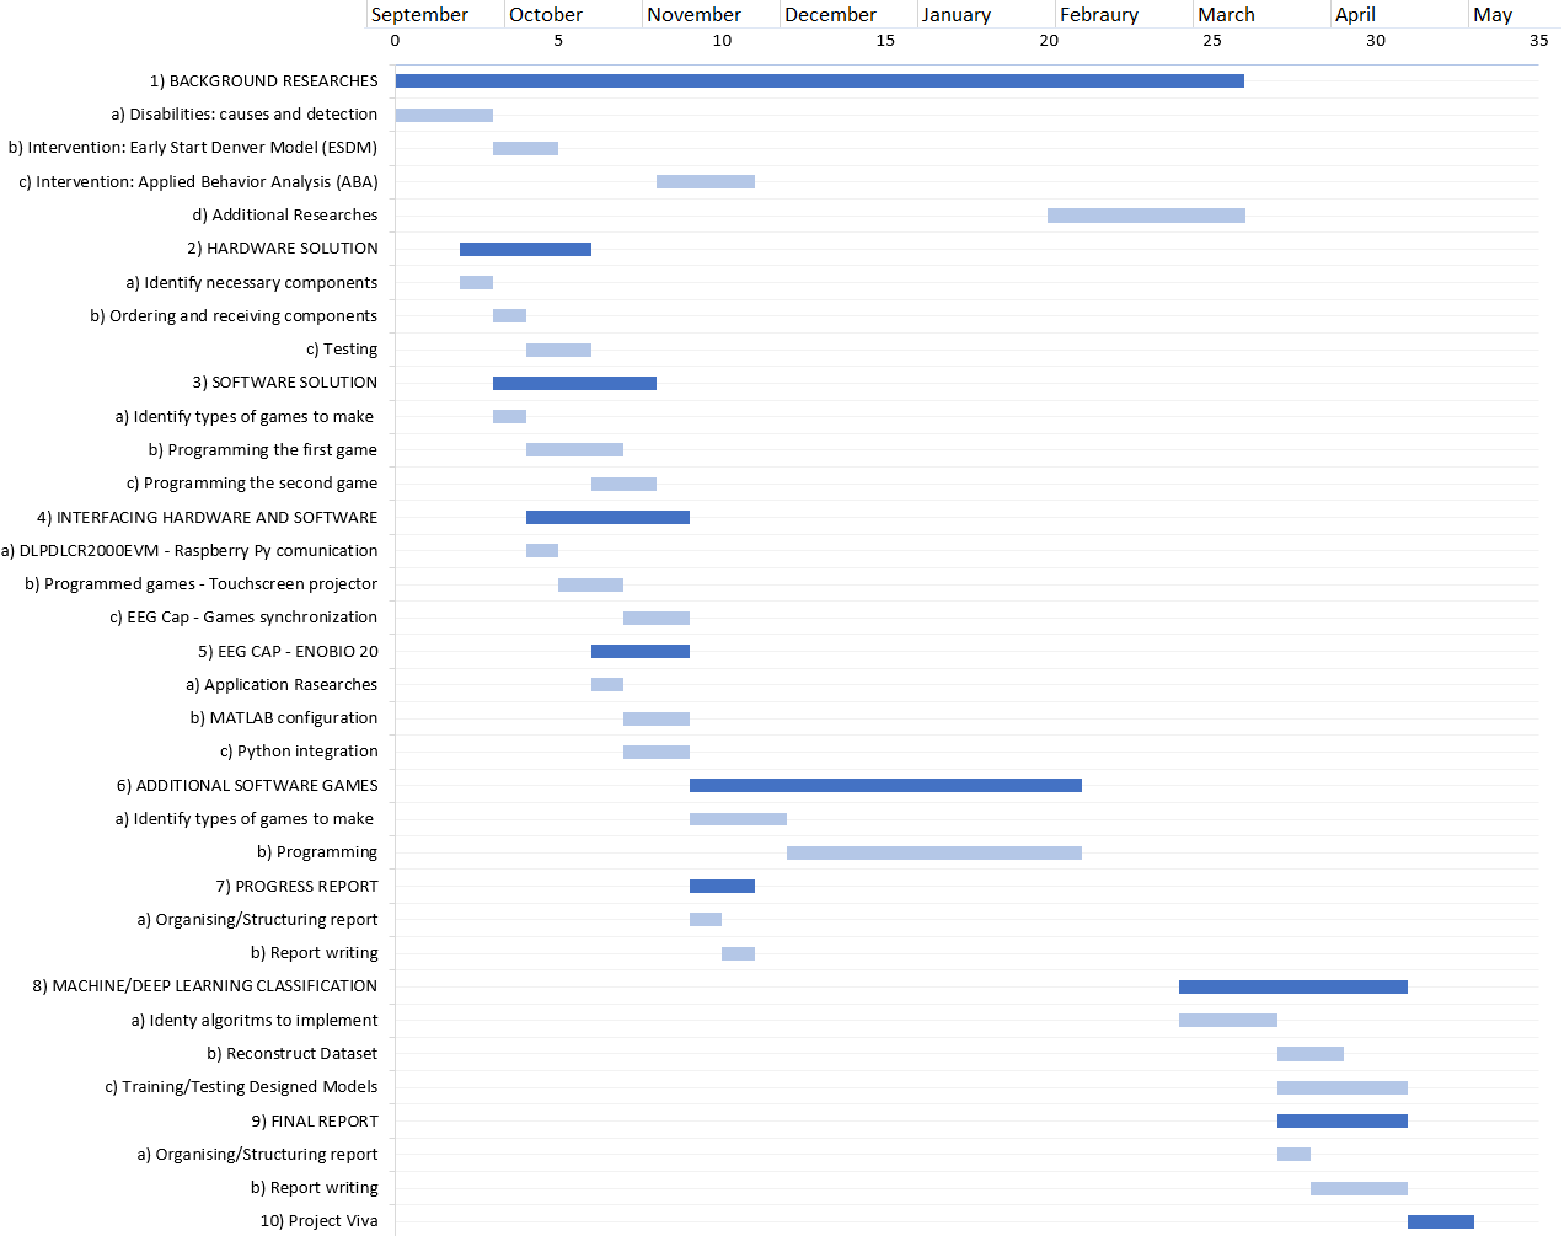
\includepdf[pages=-,pagecommand={\null\vfill\captionof{figure}{Actual Gantt Chart}},noautoscale=true,offset=0 -10, scale=0.65]{images/ganttreal.pdf}

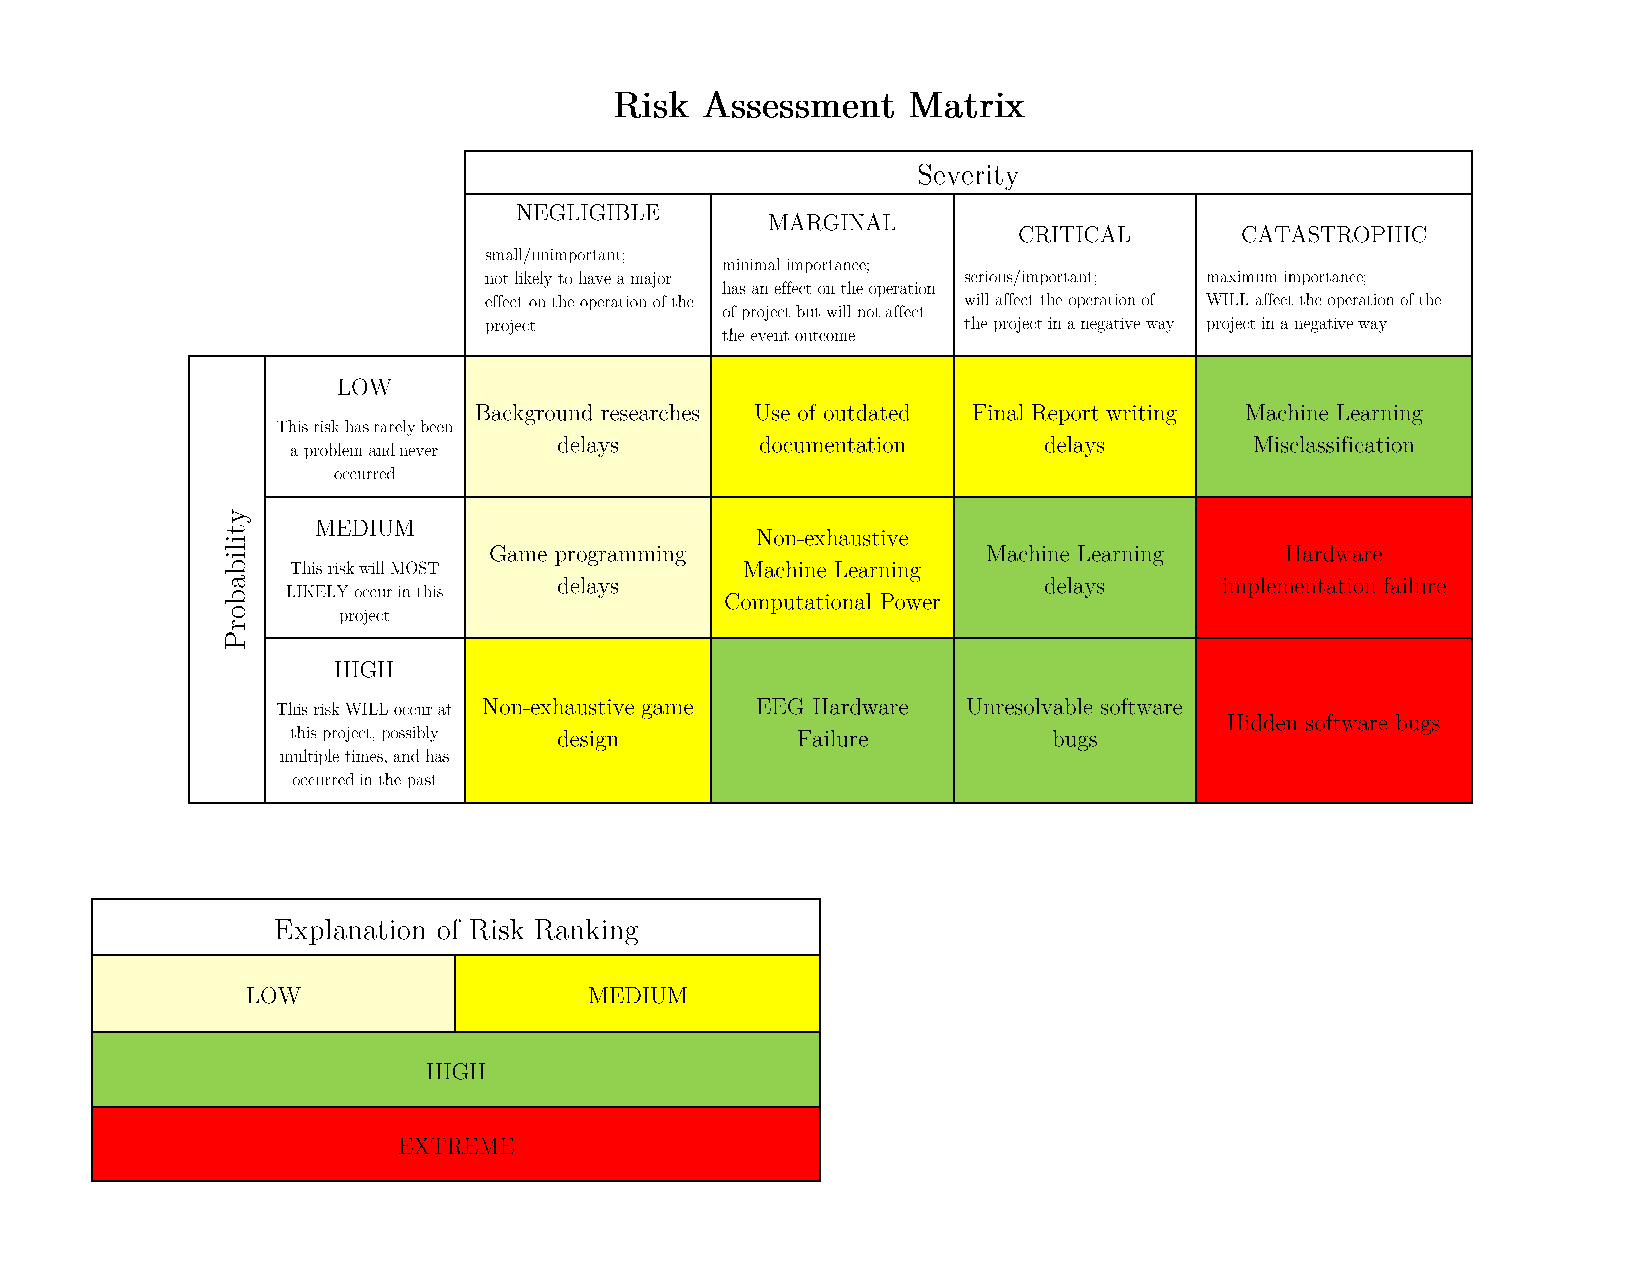
\includepdf[pages=-,pagecommand={\null\vfill\captionof{figure}{Risk Assesment Matrix}},noautoscale=true,offset=0 -10, scale=0.7]{images/Management.pdf}

\clearpage
\begin{figure}[ht!]%
    \centering
    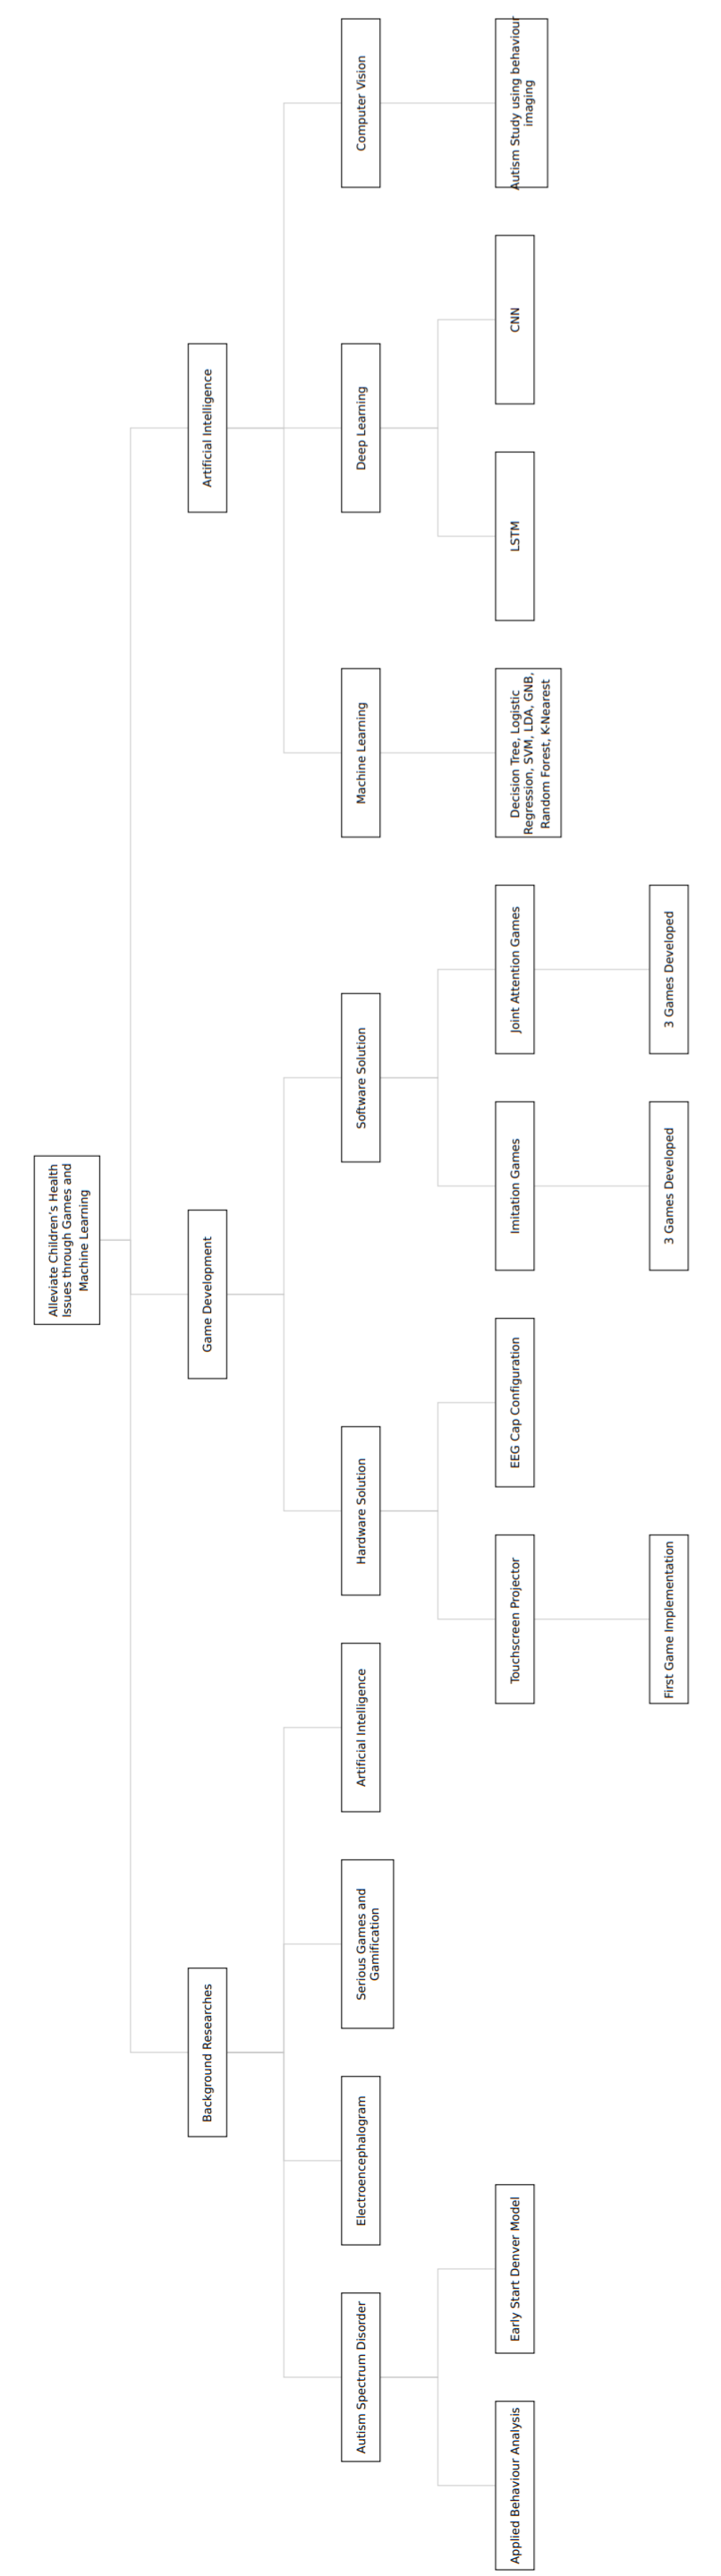
\includegraphics[width=7cm]{images/WBS1}%
    \caption{Work Breakdown Structure}%
\end{figure}

\clearpage

\setcounter{figure}{0}
\section{Evaluation Board wiring and stand}
\begin{figure}[ht!]%
    \centering
    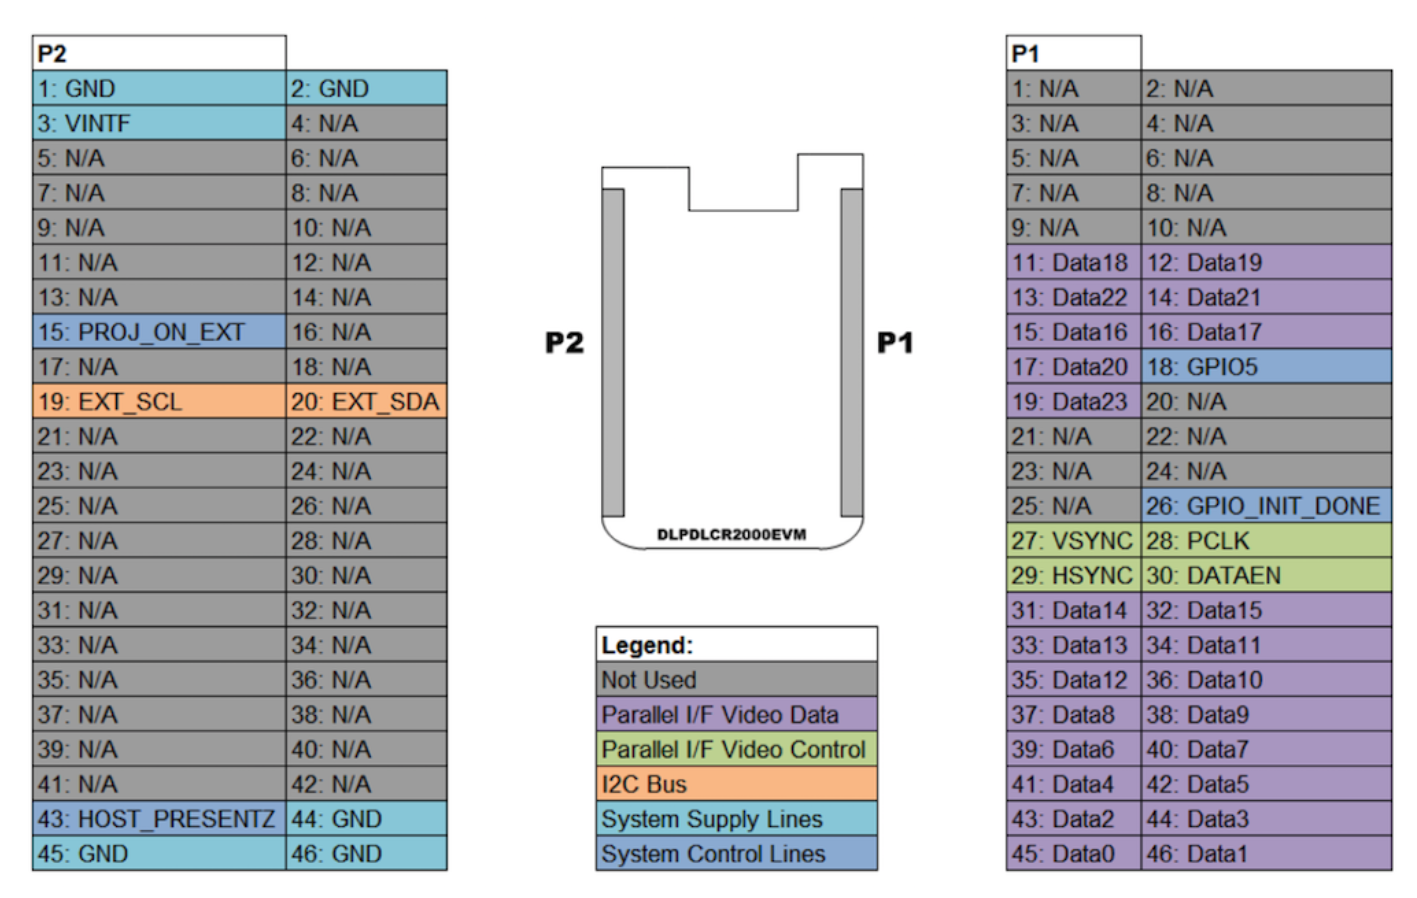
\includegraphics[width=14cm]{images/wiring1}%
    \caption{Evaluation Board}%
\end{figure}

\begin{figure}[ht!]%
    \centering
    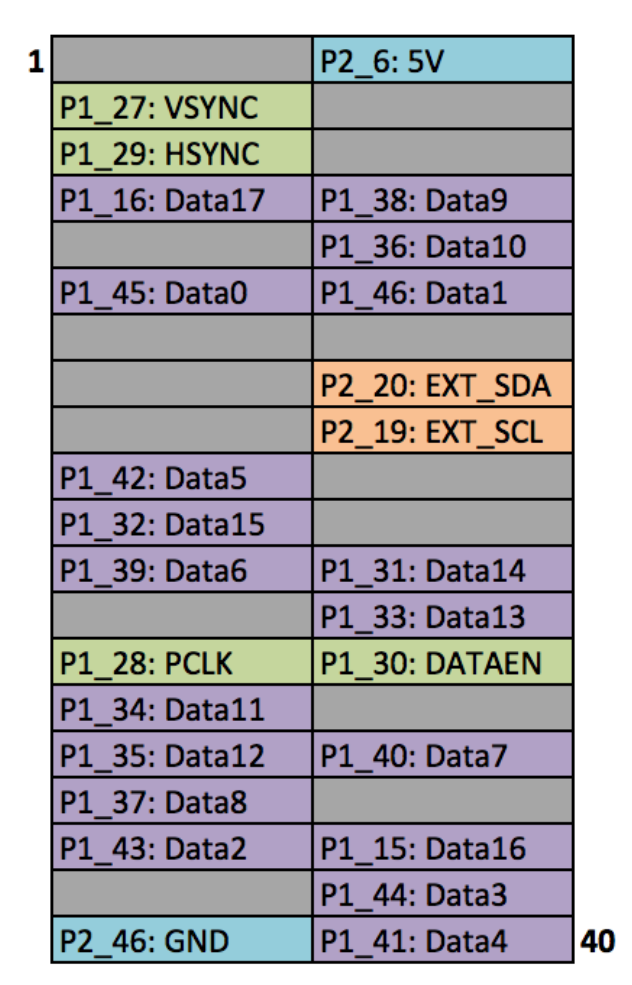
\includegraphics[width=5cm]{images/wiring2}%
    \caption{Raspberry Pi's GPIO}%
\end{figure}

Images reproduced from Frederick Vandenbosch DLP, LightCrafter Display 2000 EVM on Raspberry Pi \cite{projector}.
\clearpage

\begin{figure}%
    \centering
    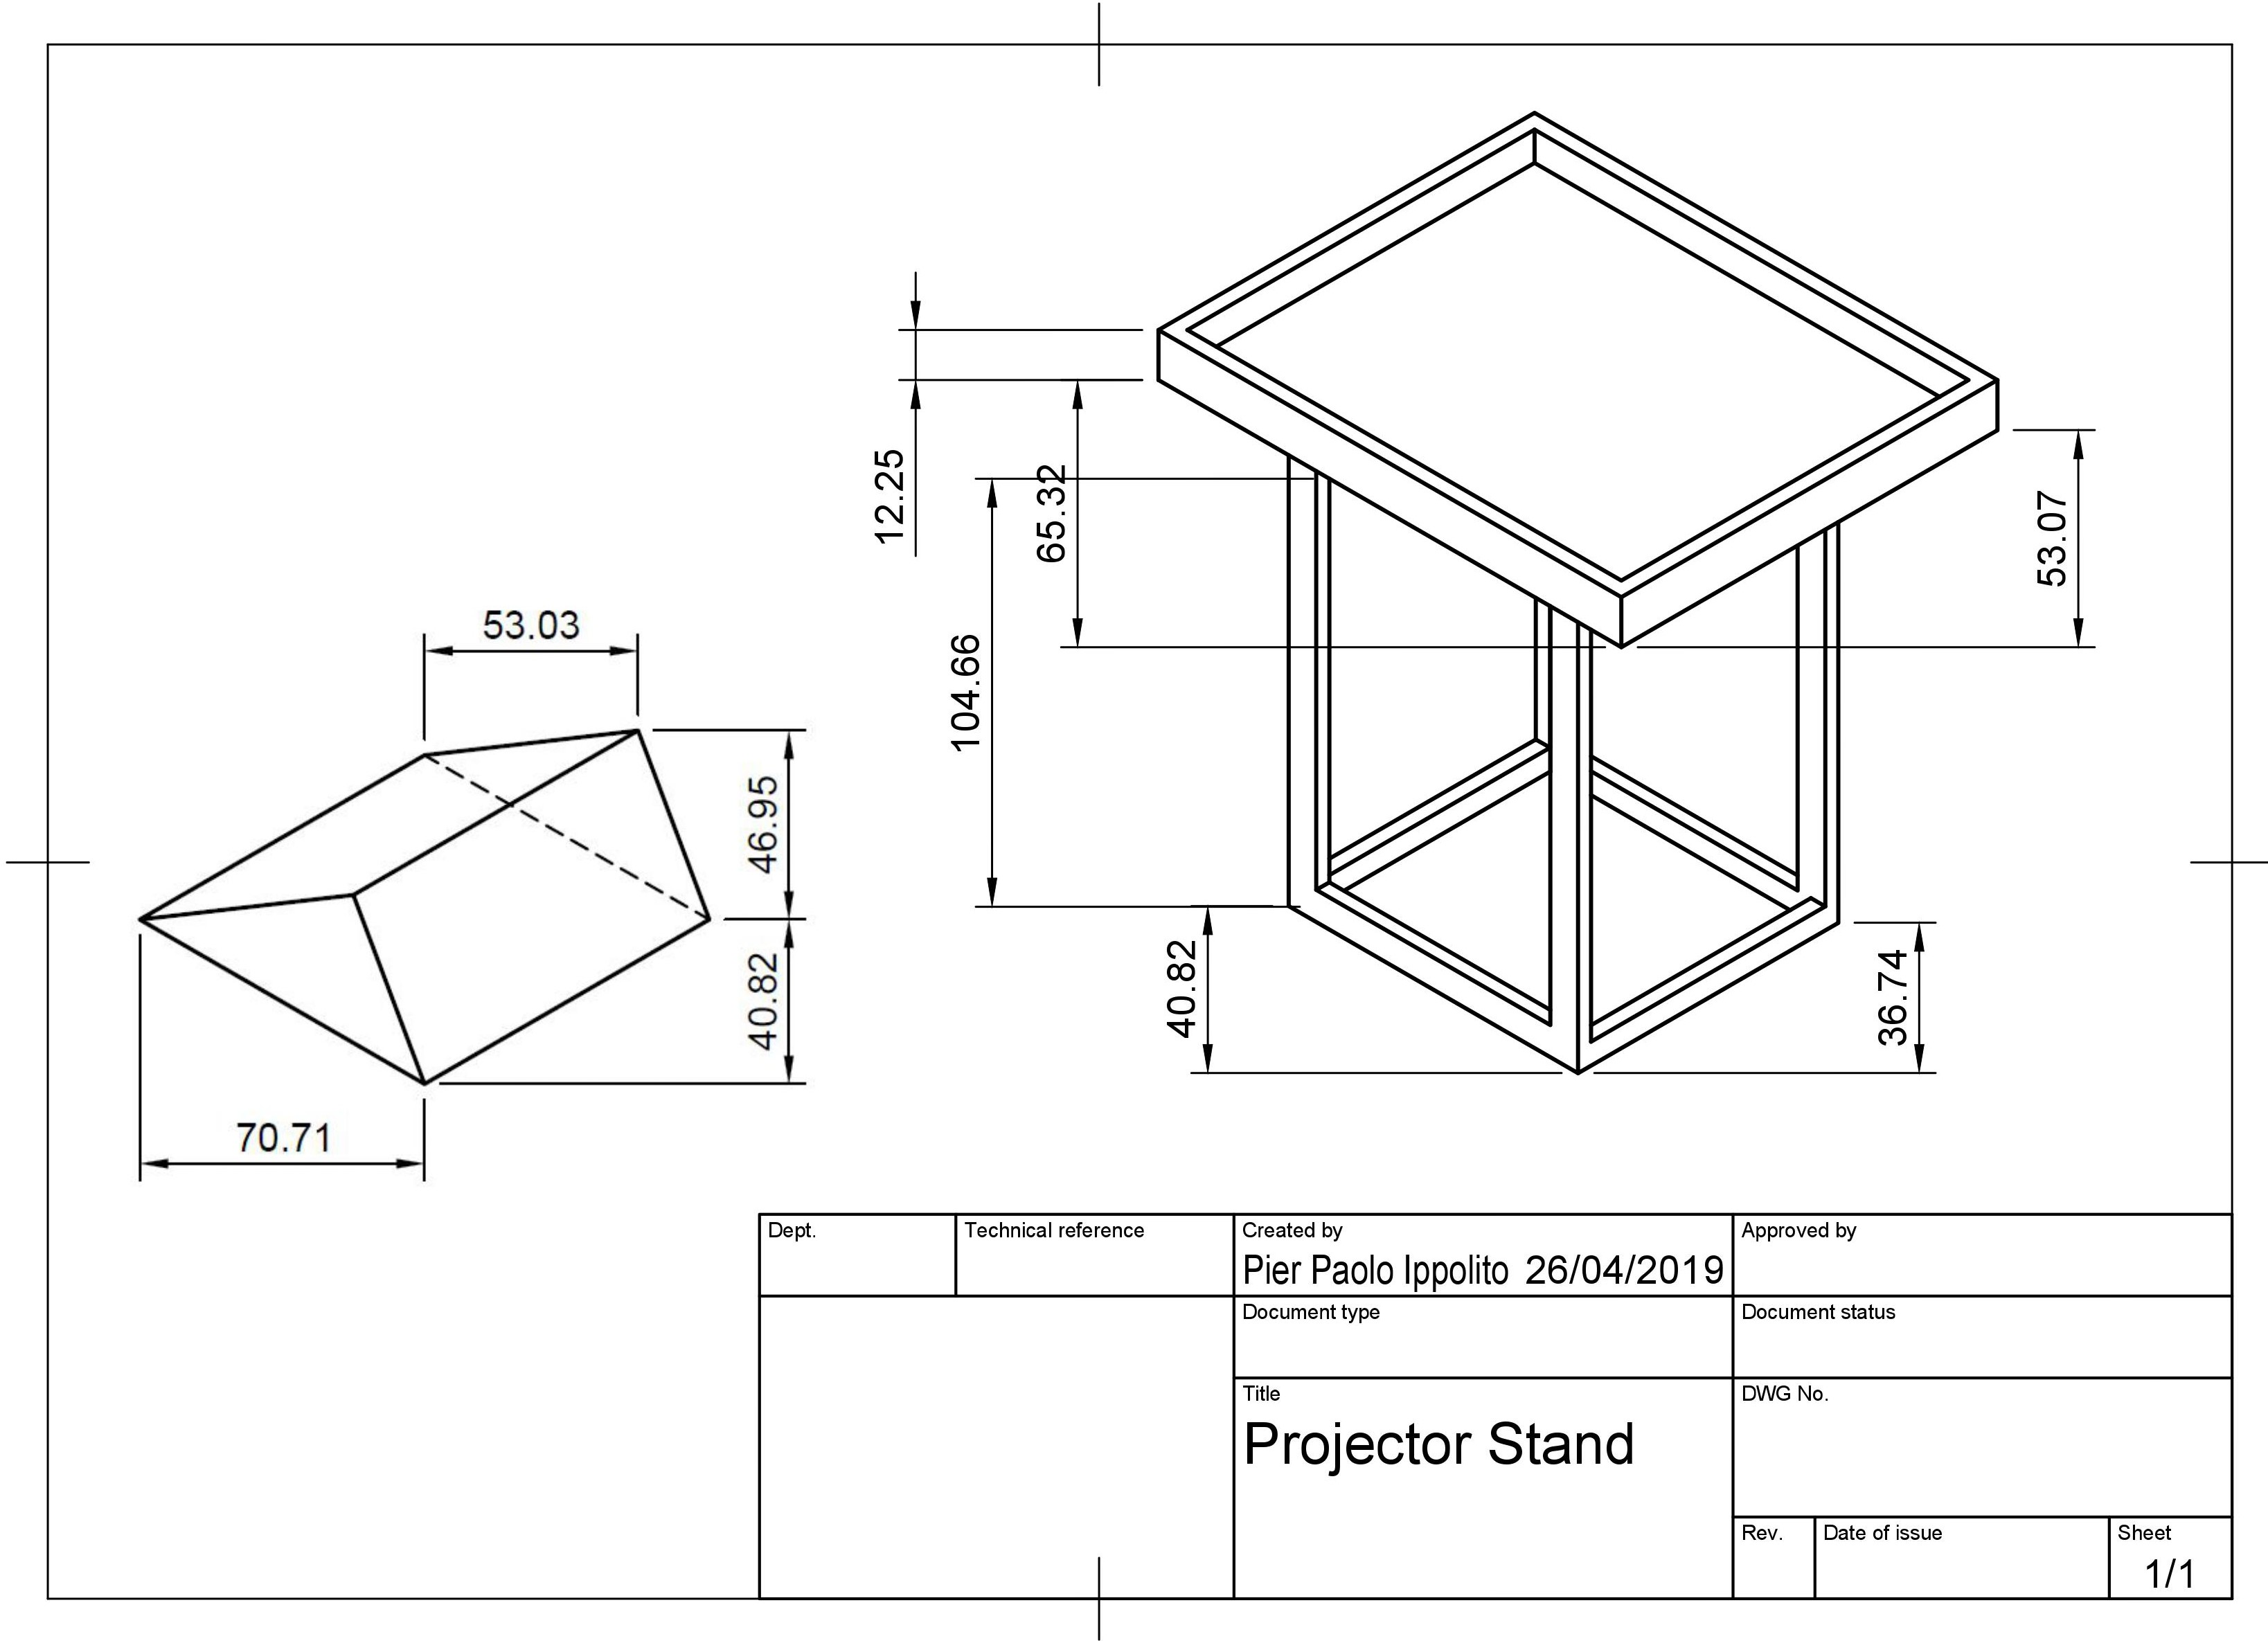
\includegraphics[width=15.3cm]{images/3d.jpg}%
    \caption{Projector stand design made using Fusion 360}%
\end{figure}

\clearpage

\includepdf[pages=-,pagecommand=\section{Project Brief},noautoscale=true,offset=0 -70, scale=1.1]{images/brief.pdf}

\clearpage
\section{Hardware Costs}

An additional risk that had to be considered at the beginning of the project, was to make best use out of the given project budget (\textsterling 150 per person). In order to make the best choice, I carried out an exhaustive research before deciding what was necessary to buy and what was not. I decided therefore, in order to limit the amount of money to spend, to make use of a Raspberry Pi 3B given to me by the University for a first year project and of a Wiimote I was already in possession before the start of the project. I also made use of other accessories necessary such as batteries, button switches and wires from the Building 16 Level 1 laboratory facilities. 

Table 1 shows the order I decided to place from the approved university supplier OneCall (Non-Marketplace). The subtotal prices column (expressed in \textsterling) takes already account of applied VAT on individual items.  

{
\begin{table}[h!]
\centering
\begin{tabular}{|c|c|c|c|}
\hline
Quantity &Description &Subtotal \\
\hline
1 & DLPDLCR2000EVM - Evaluation Board & 106.0920\textsterling \\
5 & LIR053 - Infrared Emitter - 16 °, T-1 3/4 (5mm), 20 mA & 0.9360\textsterling\\
1 & Battery Holder, AA x 1, Wire Leads & 0.8520\textsterling\\
1 & 2460 - Battery Holder, AA x 1, Through Hole & 0.8520\textsterling\\
\hline
\end{tabular}
\caption{Order Placed from Onecall (Non-Marketplace)}
\label{table:1}
\end{table}
}


At the end of the project \textsterling 41.268 out of the given budget have been saved. I planned in fact to make use of this part of the budget just in case of failure of any hardware component already acquired.

\clearpage

\clearpage
\section{Listings}

In Listing 1 has been chosen a period of 30 seconds and 20 channels.

\begin{lstlisting}[language=MATLAB, caption= MATLAB code setupscript3.m]
[ret, intletEEG] = MatNICEEGConnectLSL('NIC')
[ret, eeg_set, timestamp_set] = MatNICEEGRecordLSL(30, 20,intletEEG)
csvwrite('output-gameplay.csv',eeg_set)
\end{lstlisting}

\begin{lstlisting}[language=python, caption=Python code added to enable EEG readings synchronisation]
import matlab.engine
from threading import Thread
#  EEG readings pre-game and set-up
eng = matlab.engine.start_matlab()
eng.addpath(r'C:\Users\hp\Dropbox\Individual Project\Researches\EEG\MatNIC_v03.08', nargout=0)
tf = eng.setupscript(nargout=0)
print(tf)
# Defining threading function to get and store eeg data while playing
def eeg_func():
    # EEG readings during-game
    eng = matlab.engine.start_matlab()
    eng.addpath(r'C:\Users\hp\Dropbox\Individual Project\Researches\EEG\MatNIC_v03.08', nargout=0)
    tf3 = eng.setupscript3(nargout=0)
    print(tf3)
Thread(target = eeg_func).start() 
\end{lstlisting}

\begin{lstlisting}[language=Python, caption=Decision Tree Code]
trainedtree = tree.DecisionTreeClassifier().fit(X_Train, Y_Train)
predictionstree = trainedtree.predict(X_Test)
print(confusion_matrix(Y_Test,predictionstree))
print(classification_report(Y_Test,predictionstree))
\end{lstlisting}

\clearpage

\begin{lstlisting}[language=Python, caption=LSTM Preprocessing]
segments = []
for i in range(0, len(df) - N_TIME_STEPS, step):
    ch = []
    for j in range(0, N_FEATURES):
        ch.append(df.iloc[:, j].values[i: i + N_TIME_STEPS])
    segments.append(ch)
labels = []
for i in range(0, len(df) - N_TIME_STEPS, step):
    label = stats.mode(df['Label'][i: i + N_TIME_STEPS])[0][0]
    labels.append(label)
labelsl = np.asarray(pd.get_dummies(labels), dtype = np.float32)
reshaped_segments = np.asarray(segments, dtype= np.float32).reshape(-1, N_TIME_STEPS, N_FEATURES)
X_train, X_test, y_train, y_test = train_test_split(
        reshaped_segments, labelsl, test_size=0.2, random_state=RANDOM_SEED)
\end{lstlisting}

\begin{lstlisting}[language=Python, caption=Storing CNN Model]
model_json = model.to_json()
with open("model.json", "w") as json_file:
json_file.write(model_json)
model.save_weights("model.h5")
\end{lstlisting}

% \section{Ethics Application}

% 
\includepdf[pages={1-},scale=0.75]{images/48201_47332_FEPS_SecondaryData_01082018.pdf}


\includepdf[pages=1,scale=0.95,pagecommand={\section{Ethics Application}\label{pdf:myfile}},linktodoc=true, offset=0 -40]{images/48201_47332_FEPS_SecondaryData_01082018.pdf}

\includepdf[pages=2-,scale=0.95,pagecommand={},linktodoc=true, offset=0 -40]{images/48201_47332_FEPS_SecondaryData_01082018.pdf}

% \clearpage
% \section{ASD Screening Data Analysis for Toddlers - Behaviour Features}

% \vspace*{15pt}

% \begin{itemize}
% \itemsep0em
% \item Does your child look at you when you call his/her name?
% \item How easy is it for you to get eye contact with your child? 
% \item Does your child point to indicate that she/he wants something? (e.g. a toy that is out of reach) 
% \item Does your child point to share interest with you? (e.g. pointing at an interesting sight) 
% \item Does your child pretend? (e.g. care for dolls, talk on a toy phone)  
% \item Does your child follow where you’re looking? 
% \item If you or someone else in the family is visibly upset, does your child show signs of wanting to comfort them? (e.g. stroking hair, hugging them)
% \item Would you describe your child’s first words as:
% \item Does your child use simple gestures? (e.g. wave goodbye) 
% \item Does your child stare at nothing with no apparent purpose? 
% \end{itemize}

% List Reproduced from: Q-CHAT-10 Quantitative Checklist for Autism in Toddlers \cite{toddler}.

\clearpage
\section{ML MATLAB Analysis}

Plot of all the channels voltages registered for all the time-steps (repetition number one) in Happy Data, Typical Child number 1.

\setcounter{figure}{0}
\begin{figure}[ht!]%
    \centering
    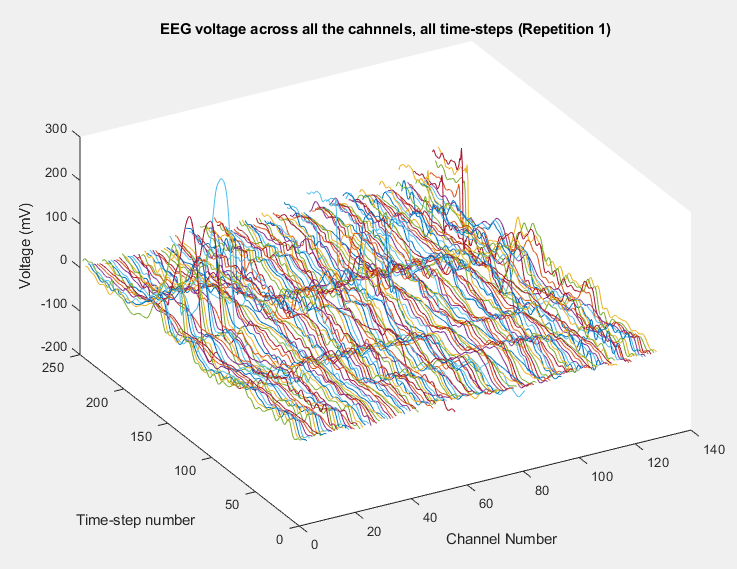
\includegraphics[width=10cm]{images/series1}%
    \caption{EEG voltage across all the cahnnels, all time-steps (Repetition 1), Happy Data, TYP1}%
\end{figure}

Plot of all the channels voltages registered for all the time-steps (repetition number one) in Happy Data, ASD Child number 1.

\begin{figure}[ht!]%
    \centering
    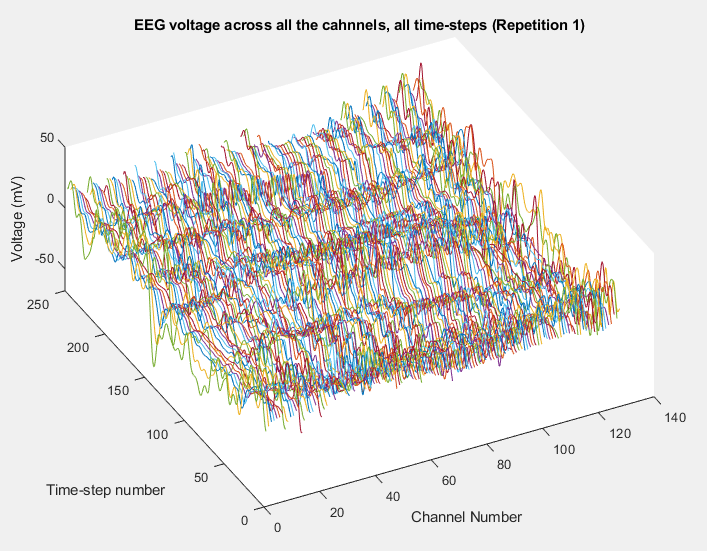
\includegraphics[width=10cm]{images/series2}%
    \caption{EEG voltage across all the cahnnels, all time-steps (Repetition 1), Happy Data, ASD1}%
\end{figure}

\clearpage

Plots of the channel number against the voltage amplitude of EEG brainwaves for the first typical child (on the left side) and the first ASD child (on the right side), this is done for all the 5 stimuli and for their corresponded experiment repetitions number 1 (left side of each plot) and 35 (right side of each plot). All the channels, all the time-steps and just one repetition is considered for each graph.

\begin{figure}[ht!]%
    \centering
    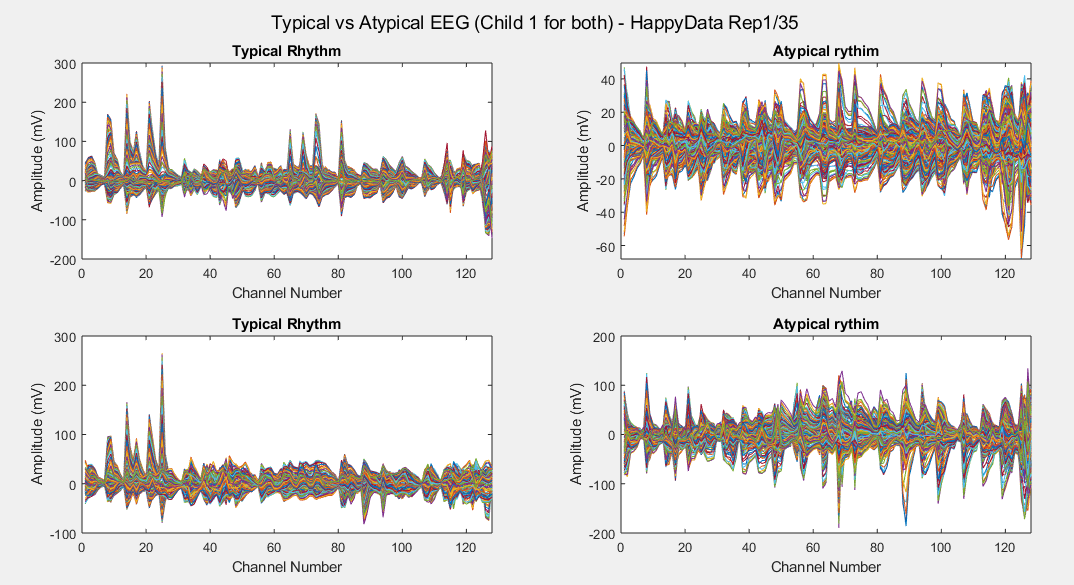
\includegraphics[width=14cm]{images/matplot1}%
    \caption{Happy Data Stimulus}%
\end{figure}

\begin{figure}[ht!]%
    \centering
    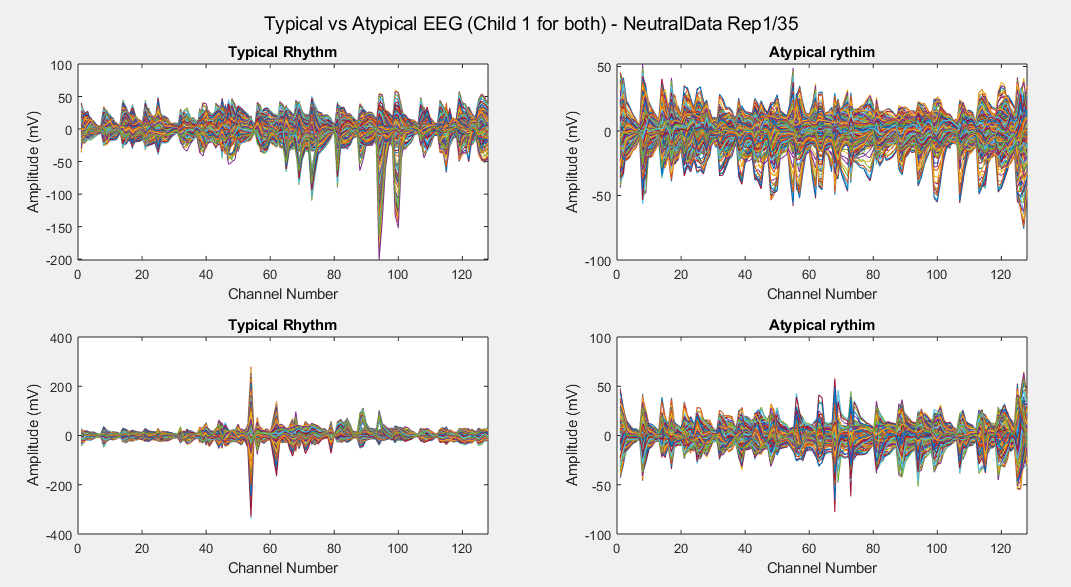
\includegraphics[width=14cm]{images/matplot2}%
    \caption{Neutral Data Stimulus}%
\end{figure}

\vspace{\floatsep}

\begin{figure}[ht!]%
    \centering
    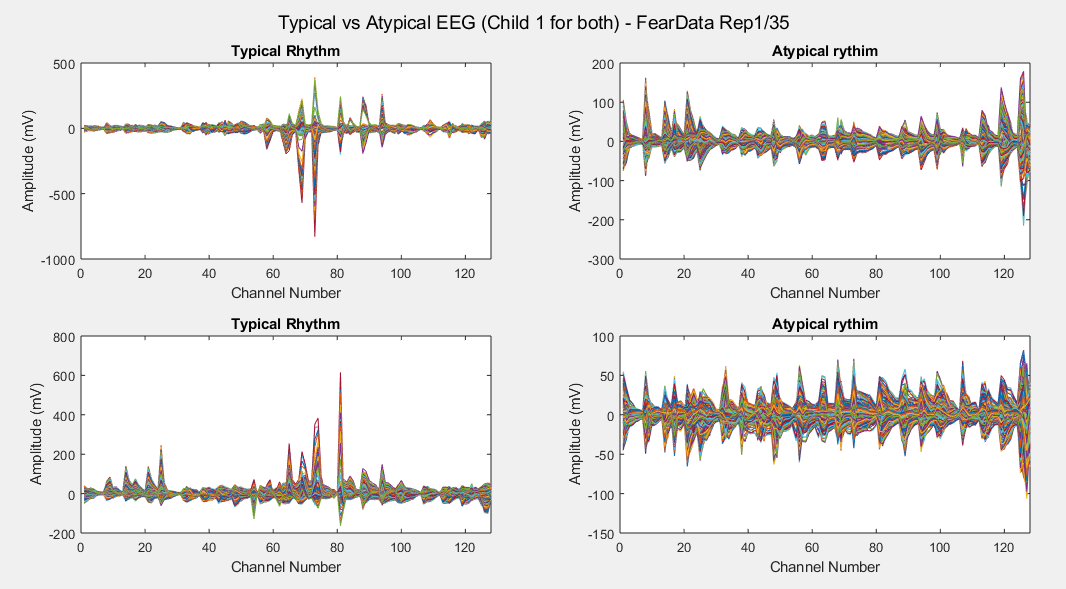
\includegraphics[width=14cm]{images/matplot3}%
    \caption{Fear Data Stimulus}%
\end{figure}

\begin{figure}[ht!]%
    \centering
    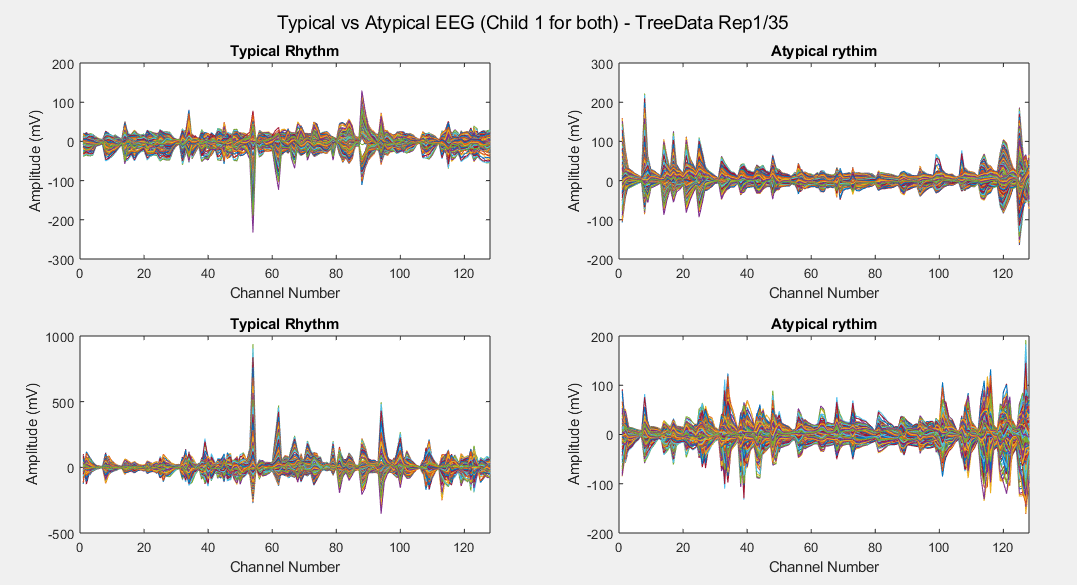
\includegraphics[width=14cm]{images/matplot4}%
    \caption{Tree Data Stimulus}%
\end{figure}

\clearpage

\begin{figure}[ht!]%
    \centering
    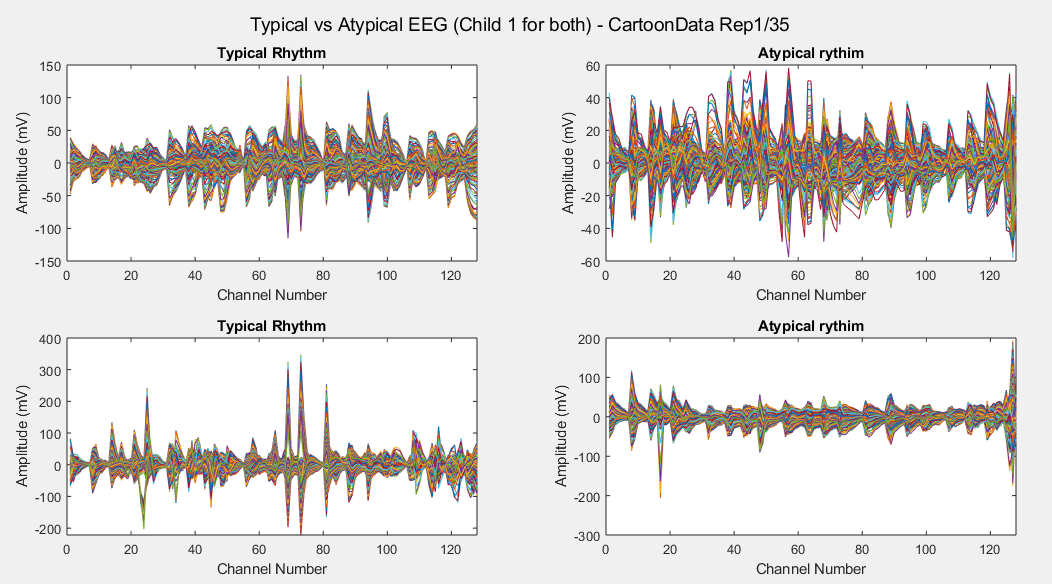
\includegraphics[width=14cm]{images/matplot5}%
    \caption{Cartoon Data Stimulus}%
\end{figure}

Considering just channel number 1, all the time-steps and just one repetition (Repetition number 1 on the left and repetition number 35 on the right of each plot), the following results can be obtained: 
\vspace{\floatsep}

\begin{figure}[ht!]%
    \centering
    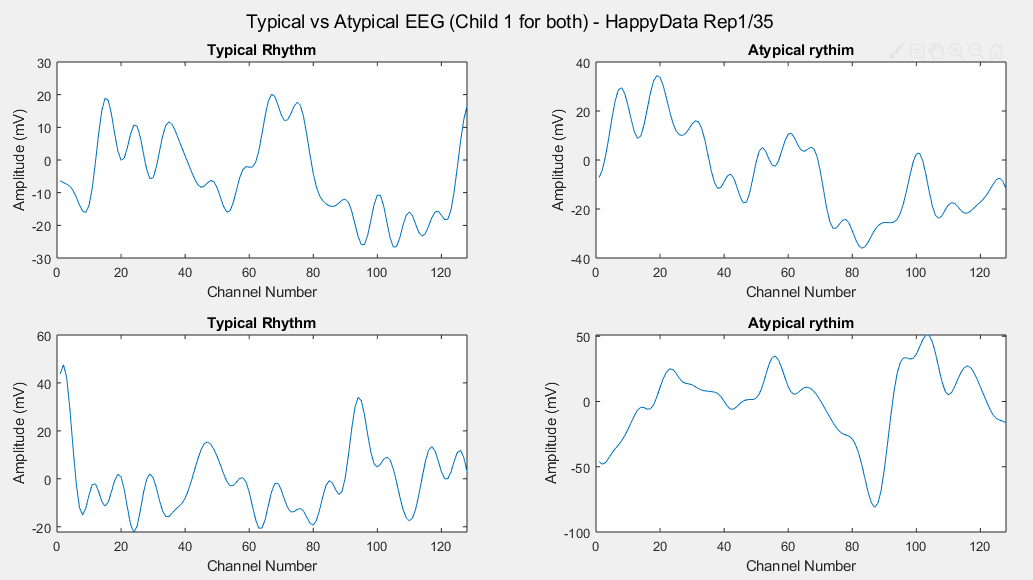
\includegraphics[width=14cm]{images/matplot6}%
    \caption{Happy Data Stimulus}%
\end{figure}

\begin{figure}[ht!]%
    \centering
    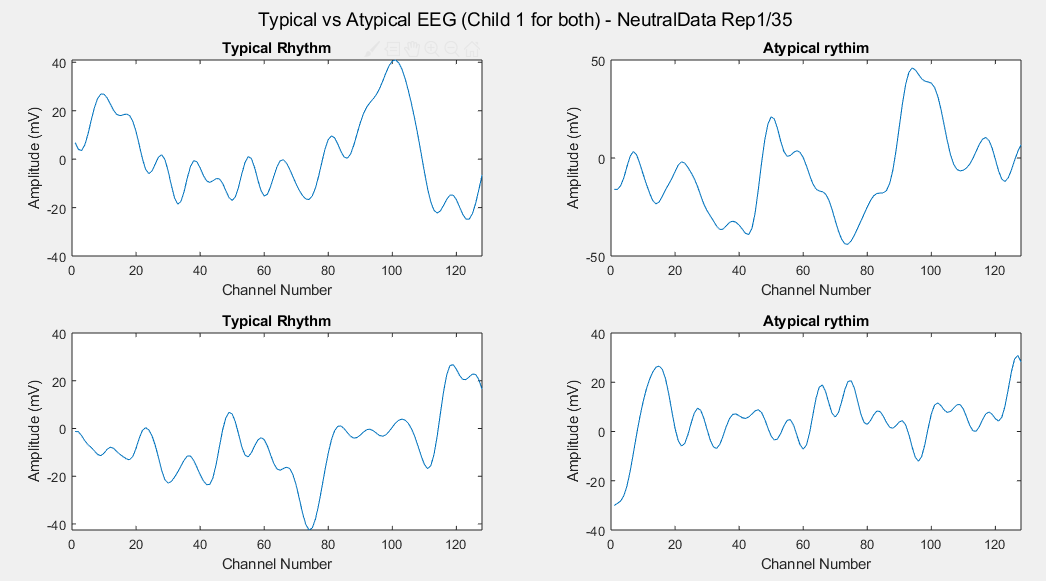
\includegraphics[width=14cm]{images/matplot7}%
    \caption{Neutral Data Stimulus}%
\end{figure}

\begin{figure}[ht!]%
    \centering
    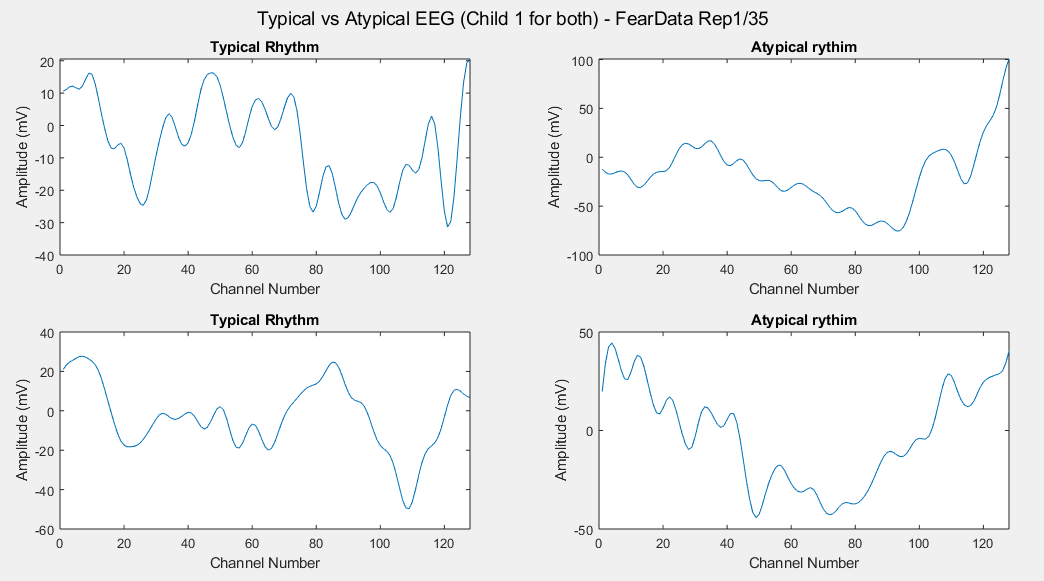
\includegraphics[width=14cm]{images/matplot8}%
    \caption{Fear Data Stimulus}%
\end{figure}

\begin{figure}[ht!]%
    \centering
    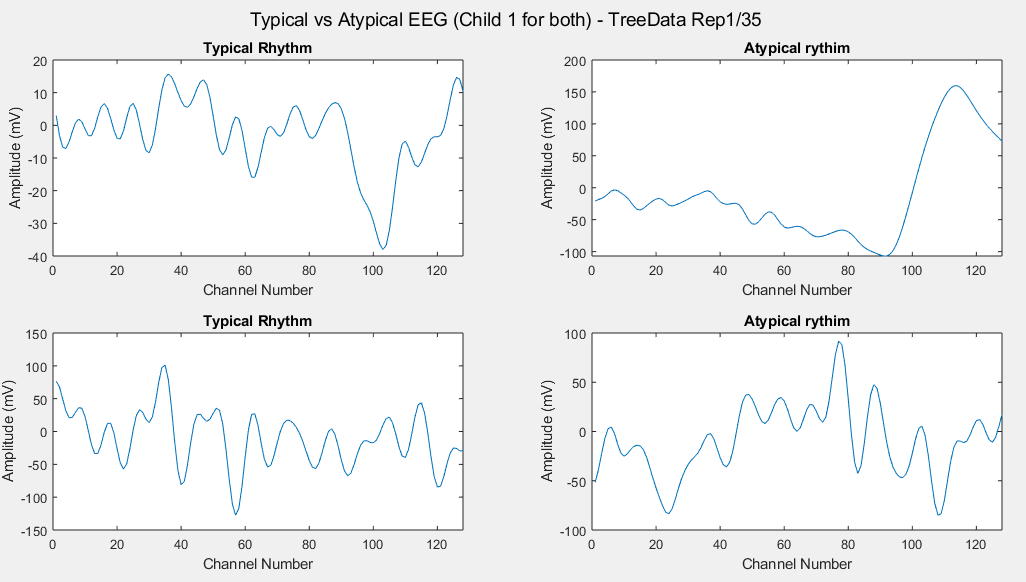
\includegraphics[width=14cm]{images/matplot9}%
    \caption{Tree Data Stimulus}%
\end{figure}

\begin{figure}[ht!]%
    \centering
    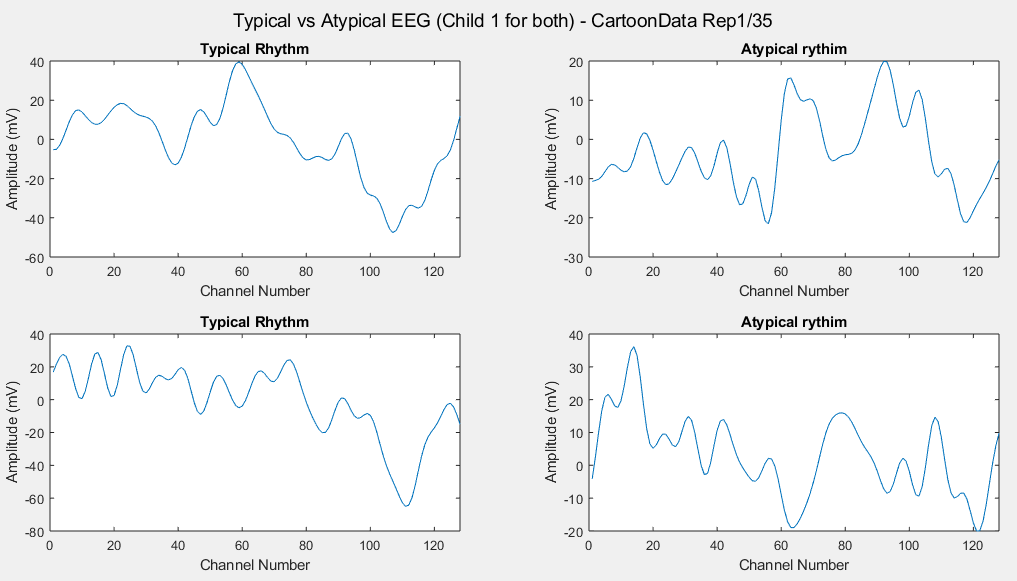
\includegraphics[width=14cm]{images/matplot10}%
    \caption{Cartoon Data Stimulus}%
\end{figure}

\clearpage
\section{Individual Stimulus Data-sets Results}
\setcounter{figure}{0}
\setcounter{table}{0}
{
\begin{table}[h!]
\centering
\begin{tabular}{|c|c|}
\hline
Data-set &Decision Tree Accuracy (\%) \\
\hline
Happy Stimulus & 79  \\
Neutral Stimulus & 80  \\
Fear Stimulus & 79  \\
Tree Stimulus & 80 \\
Cartoon Stimulus & 80 \\
\hline
\end{tabular}
\caption{Decision Tree accuracy for Individual Stimulus Data-sets}
\label{table:1}
\end{table}
}

For the LSTM because of the reduced amount of data when working with the individual stimulus, has been chosen a Train/Test split ratio of 80\% against 20\%.

{
\begin{table}[h!]
\centering
\begin{tabular}{|c|c|}
\hline
Parameter &Number \\
\hline
Time Steps & 250  \\
Features & 128  \\
Steps & 10  \\
Classes & 2 \\
Hidden Units & 64 \\
L2 Regularisation & 0.0015 \\
Learning Rate & 0.0025 \\
Epochs & 50 \\
Batch Size & 1024 \\
\hline
\end{tabular}
\caption{LSTM Parameters for Individual Stimulus Data-sets}
\label{table:1}
\end{table}
}

{
\begin{table}[h!]
\centering
\begin{tabular}{|c|c|}
\hline
Data-set &LSTM Accuracy (\%) \\
\hline
Happy Stimulus & 84.4  \\
Neutral Stimulus & 84.3  \\
Fear Stimulus & 79.5  \\
Tree Stimulus & 78.4 \\
Cartoon Stimulus & 83.1 \\
\hline
\end{tabular}
\caption{LSTM accuracy for Individual Stimulus Data-sets}
\label{table:1}
\end{table}
}

For the CNN has instead been kept a Train/Test split ratio of 70\% against 30\% and the model architecture has been slightly modified to best fit the reduced amount of data:

\begin{enumerate}
\itemsep0em
\item Two 2D Convolutional Layers having 32 filters, a kernel size of $5\times5$, a ReLU (rectified linear unit) function and the same padding. 
\item A 2D MaxPooling layer of $2\times2$ size.
\item A Dropout layer of 0.2 intensity (in order to avoid over-fitting the data)
\item A layer to first flatten the data from three dimensions to just one, and then another one to condense the input to give to the classifier 128 features (always using the ReLU function).
\item A second Dropout layer of 0.5 intensity.
\item Finally, a Dense layer (of two neurons) to produce the classification result, using a Softmax activation function.
\end{enumerate}

{
\begin{table}[h!]
\centering
\begin{tabular}{|c|c|}
\hline
Data-set &CNN Accuracy (\%) \\
\hline
Happy Stimulus & 86  \\
Neutral Stimulus & 83.2  \\
Fear Stimulus & 84.9  \\
Tree Stimulus & 78.3 \\
Cartoon Stimulus & 86.4 \\
\hline
\end{tabular}
\caption{CNN accuracy for Individual Stimulus Data-sets}
\label{table:1}
\end{table}
}

\begin{figure}[ht!]%
    \centering
    \subfloat[PCA Happy Stimulus]{{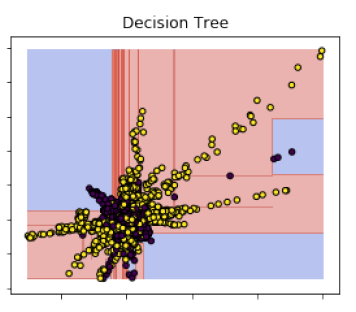
\includegraphics[width=6.7cm]{pca1} }}%
    \qquad
    \subfloat[PCA Neutral Stimulus]{{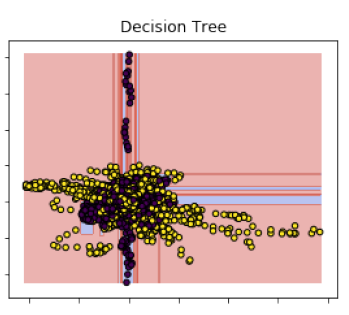
\includegraphics[width=6.7cm]{pca2} }}%
    \subfloat[PCA Fear Stimulus]{{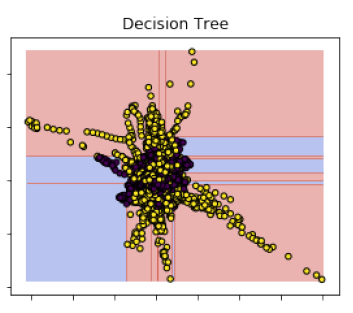
\includegraphics[width=6.7cm]{pca3} }}%
    \qquad
    \subfloat[PCA Tree Stimulus]{{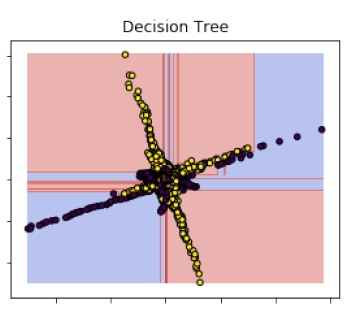
\includegraphics[width=6.7cm]{pca4} }}%
    \subfloat[PCA Cartoon Stimulus]{{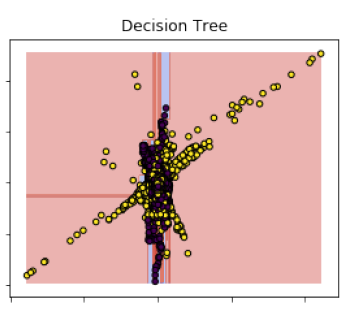
\includegraphics[width=6.7cm]{pca5} }}%
    \caption{PCA classification using Decision Tree}%
    \label{fig:example2}%
\end{figure}

\clearpage
\section{Decision Tree Classification}

The following graph was realised storing the tree as a .dot file and then using the Graphviz library. For the purposes of space, just the first 48 branches are displayed because the full decision tree is composed by more than 9000 branches. 

\setcounter{figure}{0}
\begin{figure}[ht!]%
    \centering
    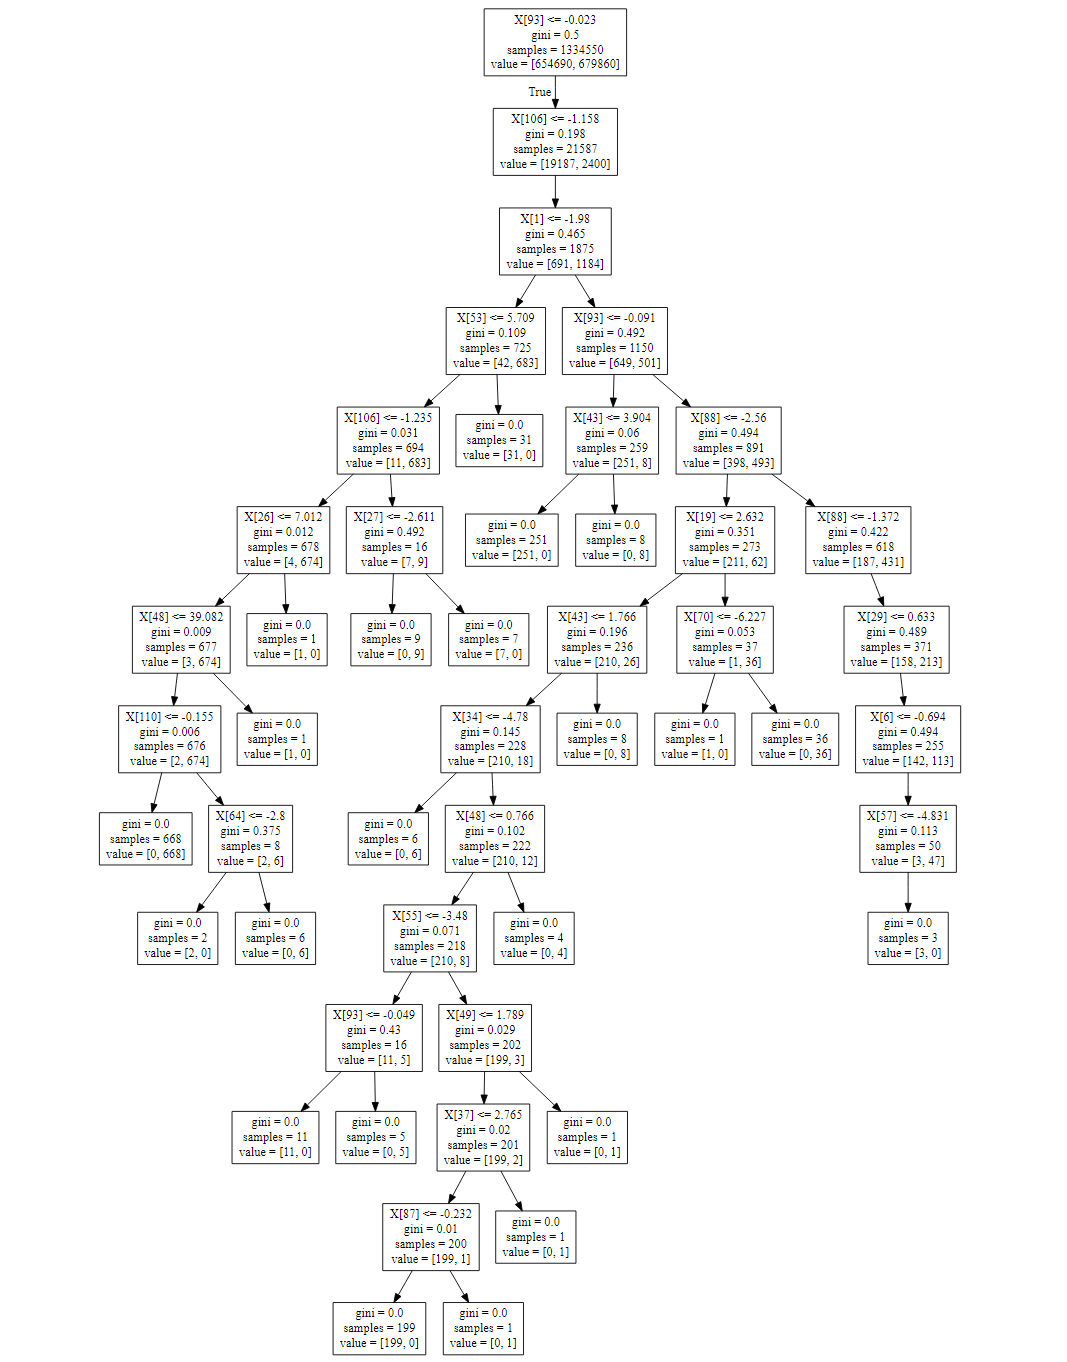
\includegraphics[width=14cm]{images/tree}%
    \caption{Decision Tree Classification Plot}%
\end{figure}

\clearpage
\section{LSTM Training/Test Loss and Accuracy}


\setcounter{figure}{0}
\begin{figure}[ht!]%
    \centering
    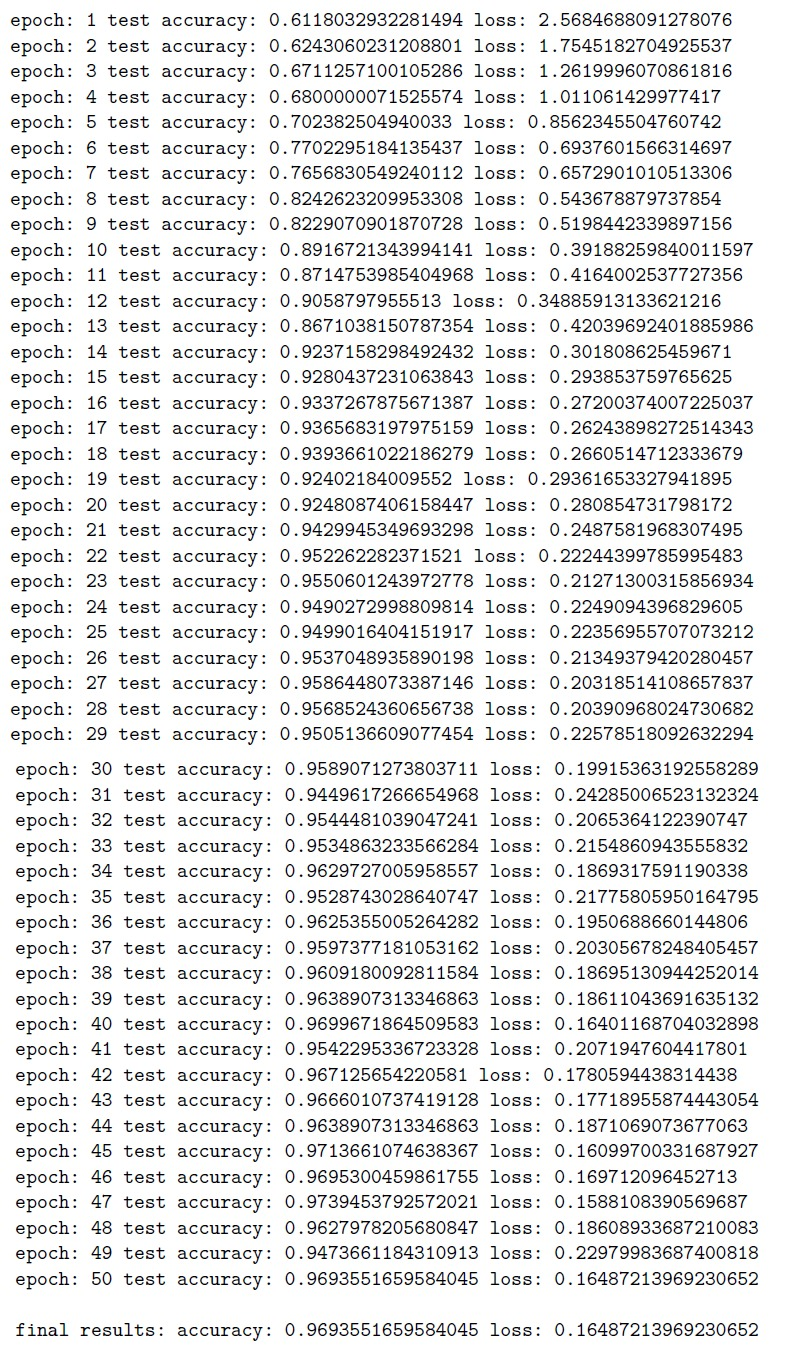
\includegraphics[width=13cm]{images/LSTMloss}%
    \caption{LSTM Training/Test Loss and Accuracy}%
\end{figure}

\clearpage
\section{Design Archive Guide}
A tree representation of this Project Design Archive is represented in Figure K.1. This image has been created through the windows command prompt using the tree command in the designed directory.
\vspace*{-17mm}
\setcounter{figure}{0}
\begin{figure}[ht!]%
    \centering
    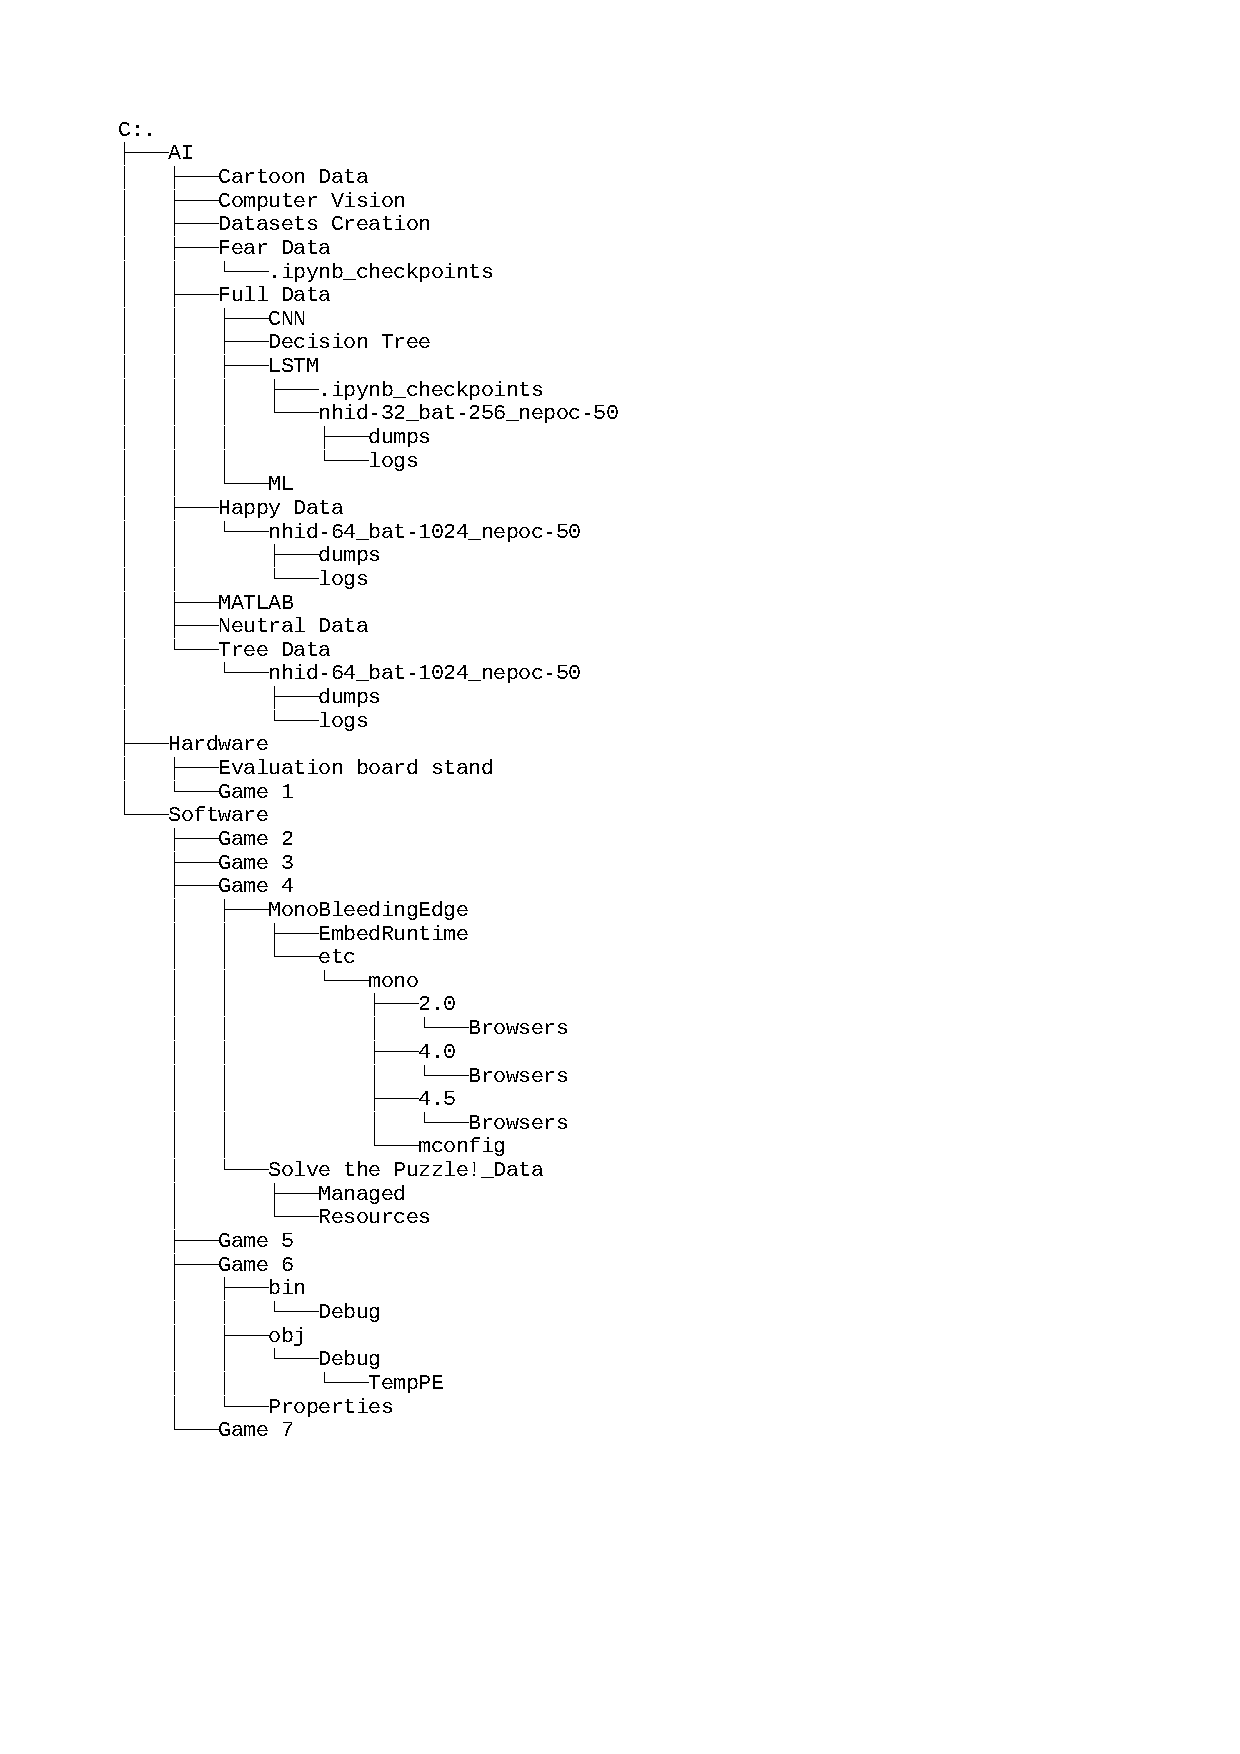
\includegraphics[page=1,scale=0.88]{images/dirtree.pdf}
    \vspace*{-52mm}
    \caption{Design Archive}%
\end{figure}

\clearpage


\section{Word Count}
%\vspace*{100pt}
The registered word count for this report, starting from Chapter 1 to Chapter 6, was equal to 9996 words. This has been measured using PDF Word Counter \cite{wordcount}.

\end{appendices}